%
% ePIC Analysis Note Template
%
% B. Surrow, January 2025
%
\includeonly{title,introduction,report,summary,ref}
%
\documentclass[12pt]{article}
%
\usepackage{hyperref}
\usepackage{lscape,longtable}
\usepackage{multirow}
\usepackage{tabularx} 
\usepackage{amsmath}  
\usepackage{comment}
\usepackage{float}
\usepackage{listings}
\usepackage{xcolor}
\usepackage{enumitem}
\usepackage{booktabs}
\usepackage{hyperref}
\usepackage{siunitx}
\usepackage{epsfig}
\usepackage{graphicx}
\usepackage{subcaption}
\usepackage[margin=1in,letterpaper]{geometry} 
\usepackage{cite} 
\usepackage{cleveref}
\usepackage{blindtext}
\usepackage{epstopdf}
\usepackage{afterpage}
\usepackage{fancyvrb}
\usepackage{fancyhdr}
\usepackage{chngcntr}
%
\setlength{\topmargin}{0.0in}
\setlength{\headheight}{0in}
\setlength{\headsep}{0in}
\setlength{\textheight}{9.05in}
\setlength{\textwidth}{6.525in}
\setlength{\oddsidemargin}{-0.0in}
\setlength{\evensidemargin}{-0.0in}
\setlength{\parindent}{0.25in}
\setlength{\parskip}{0.25in}
%
\begin{document}
%
\pagestyle{empty}
%
%
\vspace*{0.1cm}
\begin{center}
{\bf\Large ePIC Analysis Note: \# } \\
\vspace*{1.0cm}
{\bf\Large Title Goes Here} \\
\vspace*{0.5cm}
{\bf\Large 2nd Line of Title} \\
\end{center}
%
\vspace*{1.0cm}
%
\begin{center}
{\bf Principal Author List:} \\ 
\vspace*{0.25cm}
Author 1 (Institution, Email)\\
Author 2 (Institution, Email)\\
Author 3 (Institution, Email)\\
Author 4 (Institution, Email)\\
Author 5 (Institution, Email)\\
\end{center}
%
\date{\today}
%
\pagebreak
%
\begin{abstract}
\noindent Abstract for analysis note goes here.
 \end{abstract}
%
\pagenumbering{roman}
\pagestyle{plain}
\setcounter{page}{3}
\tableofcontents
\cleardoublepage
\listoffigures
\cleardoublepage
%
\listoftables
\cleardoublepage
%
\pagenumbering{arabic}
\pagestyle{plain}
%
\setcounter{page}{6}
%
\section{Introduction}\label{sec:introduction}

\noindent \textit{Brief introduction to the physics motivation of the analysis presented here (1-2 pages). Here is an example plot shown in Figure~\ref{Fig1}. Here is an example for a reference~\cite{AbdulKhalek:2021gbh}.}

\begin{figure}[H]
\centerline{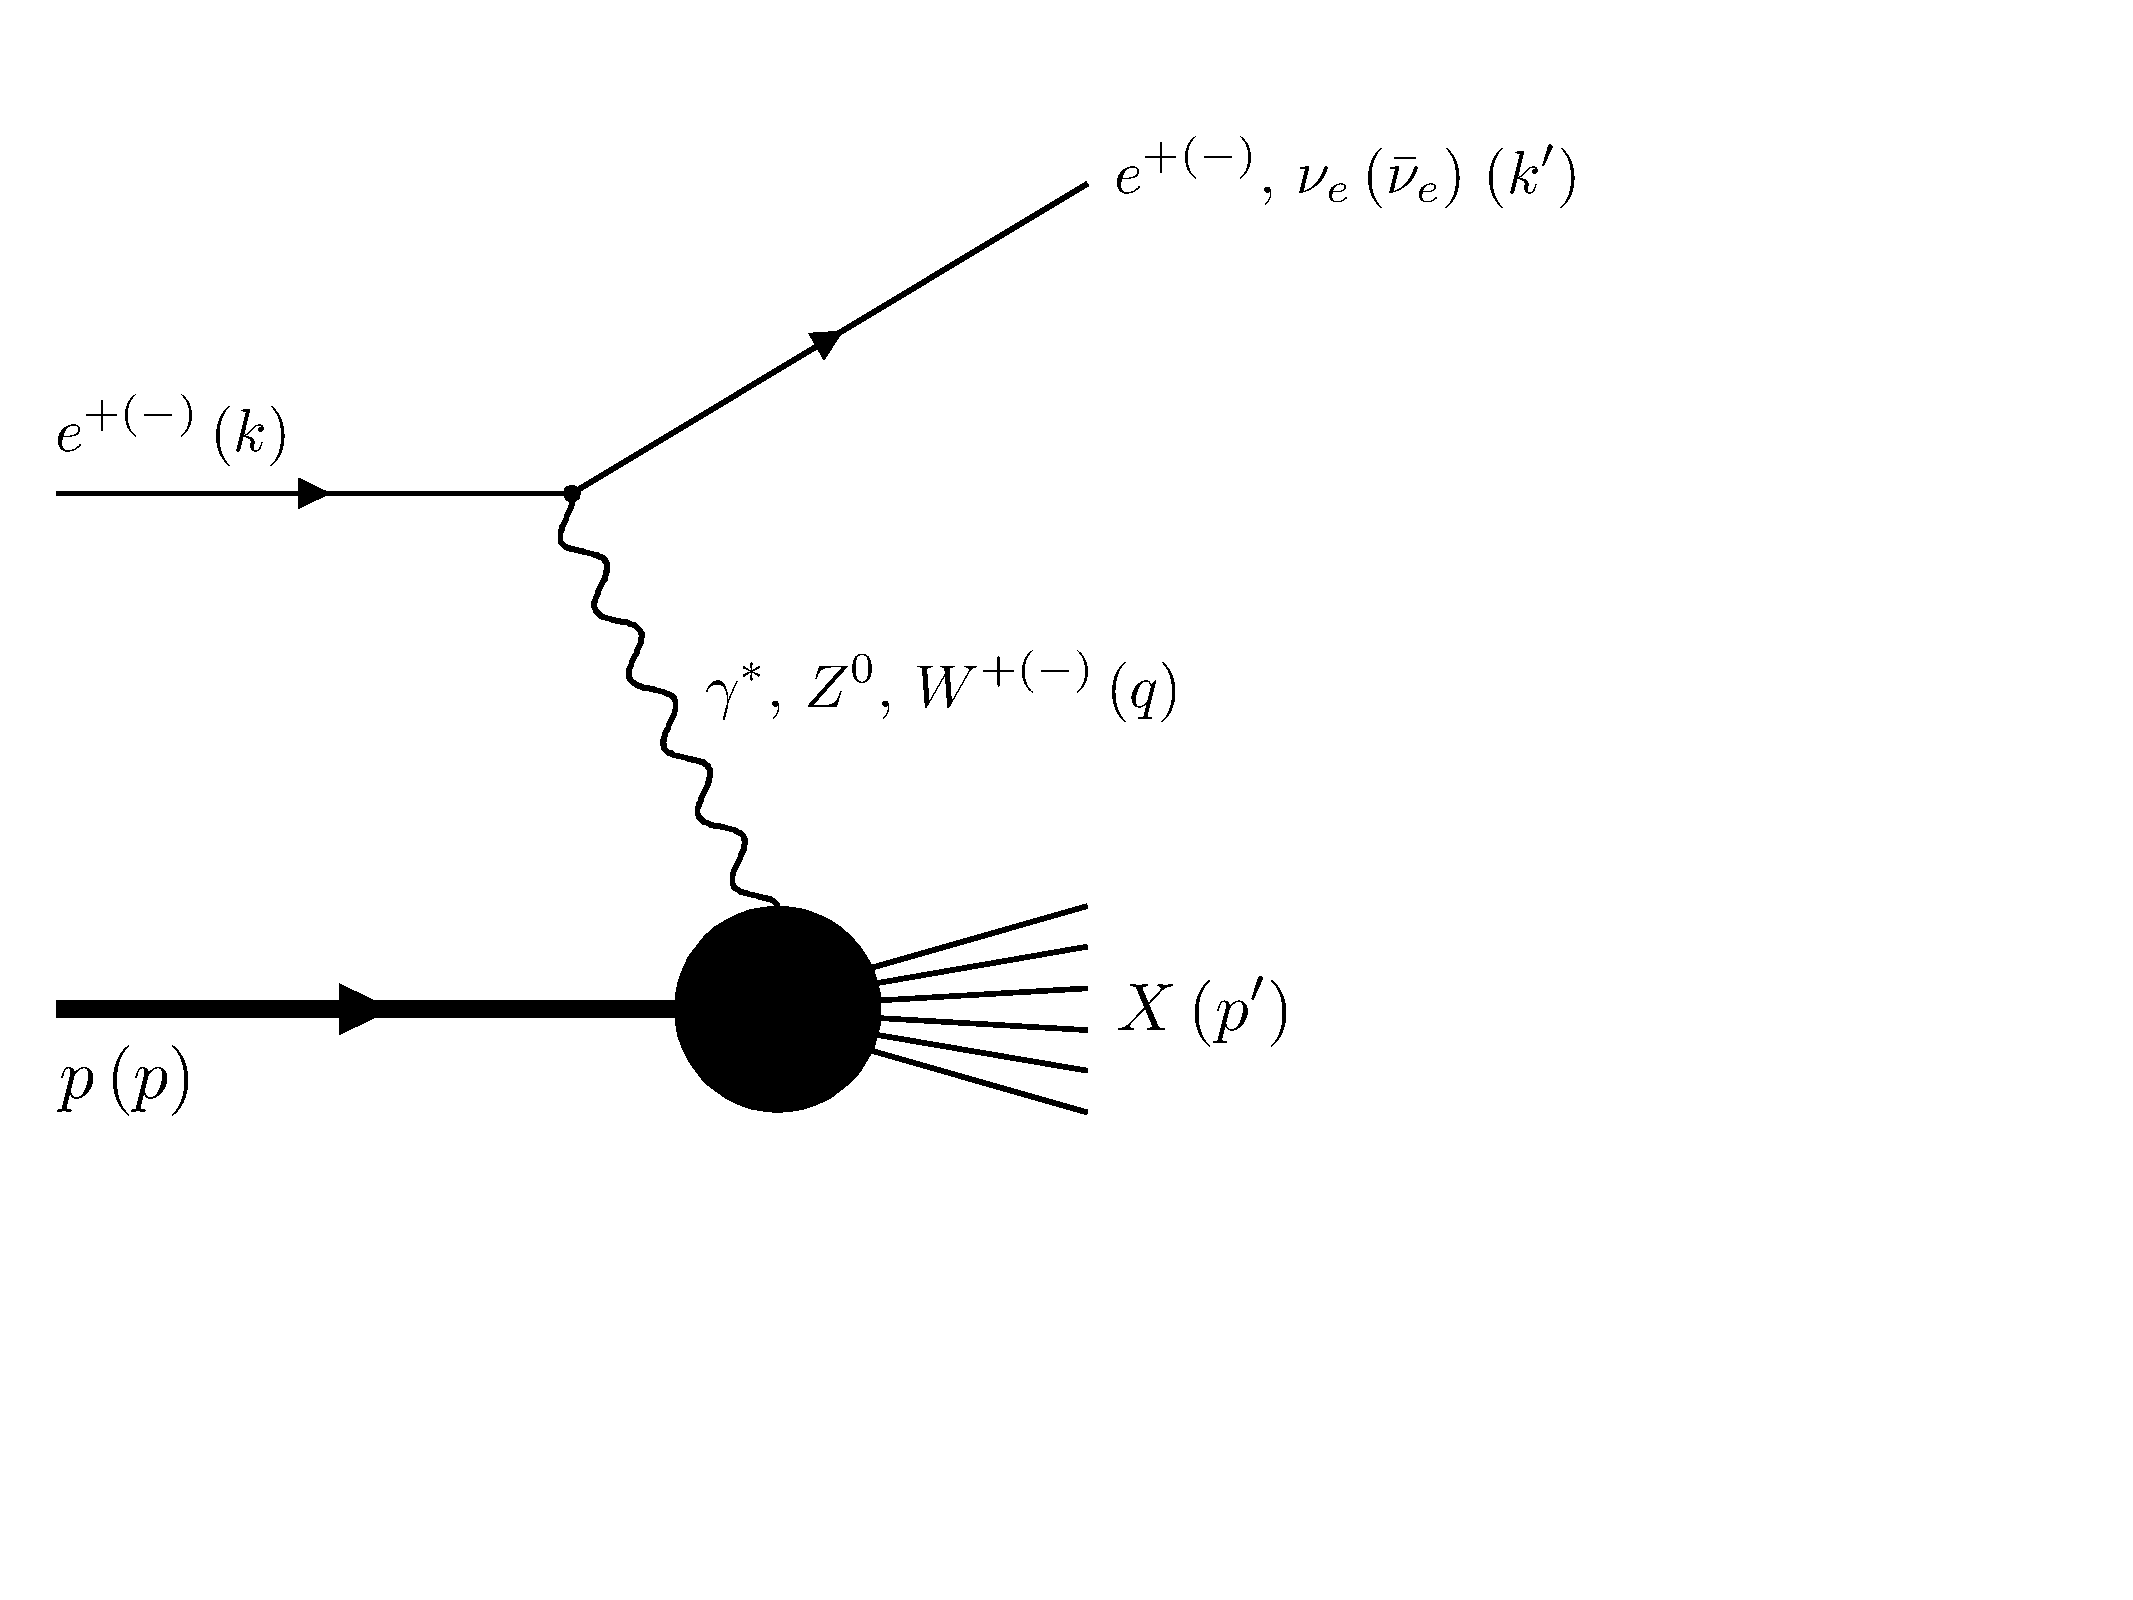
\includegraphics[width=65mm]{ep_Feynman_graph}}
\caption[Figure 1 text]{\it Feynman graph for $ep$ scattering.}
\label{Fig1}
\end{figure}

\section{Analysis details}\label{sec:report}
\textit{Sufficient information on the analysis should be provided such that other ePIC members, if desired, are able to reproduce the results by following this analysis note and utilizing associated analysis codes. }

\subsection{Data and Monte Carlo Samples}
\textit{Description of the data and simulation samples used in this analysis. Please include sufficient details, such as software version used for data production or special calibration files, so readers can easily identify them.}

\subsection{Event, Particle and PID Selections}
\textit{Description of how events (type, vertex, kinematics, etc) and particles (tracks, clusters, hits, etc) are selected. PID information, if used, should be elaborated as well.}

\subsection{Signal Extraction}
\textit{Detailed description of how raw signals are reconstructed and extracted.}

\subsection{Corrections for Detector Effects}
\textit{Detailed description of the correction scheme for detector acceptance, efficiency, resolution, etc.}

\subsection{Systematic Uncertainties}
\textit{Detailed description of how systematic uncertainties are evaluated. Figures and/or tables are recommended to illustrate the magnitudes of different uncertainty sources and their evolution with measured observables. Correlations of uncertainties should also be discussed.}

\subsection{Results and Discussions}
\textit{Presentation of all the results derived from this analysis, including figures, tables, confidence level, etc. Associated physics messages should be included as well. }

\noindent\textit{Here is an example: Table~\ref{Table1}.}

\begin{table}[h]
    \centering
    \begin{tabular}{ccccc}
        \toprule
        $x$ & $Q^{2}$ (GeV$^{2}$) & $F_{2}$ & Stat. Error & Syst. Error \\
        \midrule
        0.001 & 1.2 & 0.345 & 0.012 & 0.023 \\
        0.005 & 2.3 & 0.512 & 0.015 & 0.030 \\
        0.010 & 3.1 & 0.678 & 0.018 & 0.035 \\
        0.020 & 4.7 & 0.823 & 0.020 & 0.040 \\
        0.030 & 5.8 & 0.912 & 0.022 & 0.045 \\
        0.050 & 6.2 & 1.034 & 0.025 & 0.050 \\
        0.070 & 7.1 & 1.189 & 0.027 & 0.055 \\
        0.100 & 8.3 & 1.245 & 0.030 & 0.060 \\
        0.200 & 9.5 & 1.387 & 0.033 & 0.065 \\
        0.300 & 10.0 & 1.456 & 0.035 & 0.070 \\
        \bottomrule
    \end{tabular}
    \caption[Text for Table 1]{\it Example table of $x$, $Q^{2}$, $F_{2}$ values (Random values!) with statistical and systematic errors.}
    \label{Table1}
\end{table}

\section{Summary}\label{sec:summary}

\noindent \textit{Briefly summarize the main findings of the analysis.}


%
\bibliographystyle{h-physrev3}
\bibliography{reference}
%
\end{document}
%